\chapter{Testovanie FSFSODT}\label{chap:previous_solutions}
V predošlej kapitole sme si popísali ako funguje prístup metódy Frustratingly simple few shot object detection \cite{FSFSODT}. Teraz si ju prakticky vyskúšame a otestujeme pre rôzny počet trénovacích obrázkov pre novel classes. A taktiež ako sa s ňou dá reálne pracovať a ako je rýchla posledná fáza tréningu fine-tuning pri trénovaní na jednom GPU konkrétne NVIDIA RTX 3070. 

\section{Dataset}
Ako prvé bolo potreba zvoliť a pripraviť dataset na ktorom budem túto metódu testovať. Zvolil som si veľmi známy dataset PASCAL VOC~\cite{VOC}, ktorý sa bežne používa pre porovnanie presnosti medzi rôznymi algoritmami. Tento dataset obsahuje 20 tried. 

Pri few-shot object detection, potrebujeme mať dataset rozdelený na triedy ku ktorým máme veľké množstvo anotovaných dát (base classes), a na triedy ku ktorým máme malé množstvo anotovaných dát (novel classes).

Ako base classes som použil triedy: aeroplane, bicycle, boat, bottle, car, cat, chair, diningtable, dog, horse, person, pottedplant, sheep, train, tvmonitor.

Ako novel classes som použil triedy z PASCAL VOC:
bird, bus, cow, motorbike, sofa a taktiež som pridal jednu vlastnu triedu apple (anotované obrázky som stiahol z roboflow~\cite{roboflow}) príklady anotovaných obrázkov pre túto triedu môžme vidieť na obrázku \ref{fig:image401}.

Keďže tvorcovia poskytli predtrénované modely, časovo a výpočtovo najnáročnejšiu prvú fázu tréningu base tréning som mohol vynechať, keďže používam rovnaké base classes dopadla by úplne rovnako a jej výstup môžem použiť pre následný fine tuning pre rôzne novel classes a aj pre rôzny počet anotovaných obrázkov pre novel classes. 

Najprv treba stiahnúť PASCAL VOC dataset a umiesniť ho do priečinka \texttt{datasets} následne pridať do \texttt{datasets/VOC2007/Annotations} anotácie novo pridanej triedy, do \texttt{datasets/VOC2007/JPEGImages} obrázky tejto novej triedy a následne do \texttt{datasets/VOC2007/ImageSets/Main/trainval.txt} pridať názvy obrázkov, ktoré budeme chcieť použiť na tréning (fine tuning) a zvyšné názvy obrázkov pridáme do \texttt{datasets/VOC2007/ImageSets/Main/test.txt}, ktoré budú použité na testovanie. 

Následne bolo treba pripraviť textové súbory pre každú triedu, ktoré obsahovali názvy obrázkov pre rôzny k-shot fine tuning, k-shot fine tuning znamená, že budem robiť fine tuning na k anotovaných obrázkoch pre každú novel triedu. Teda k obrázkov bude použitých na tréning a validáciu počas fine tuningu. Tieto textové súbory musia byť umiestnené v \texttt{datasets/vocsplit} pre ich generovanie môžme použiť script \texttt{datasets/prepare\_voc\_few\_shot.py}


\begin{figure}[H]
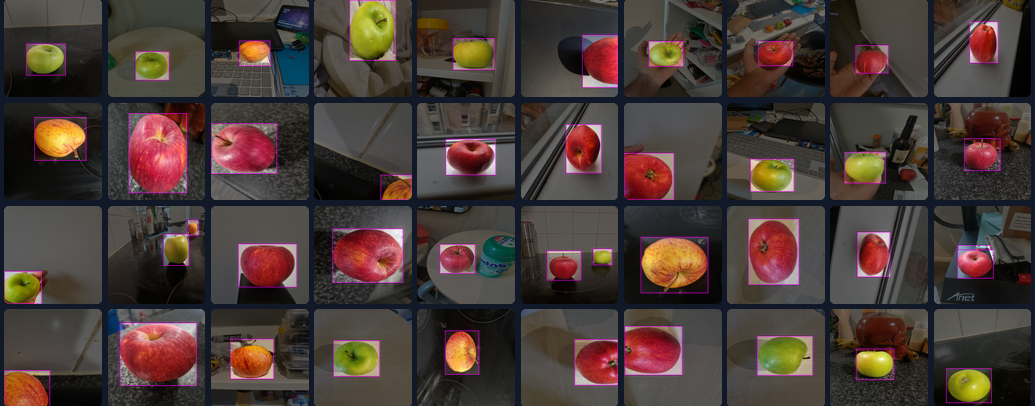
\includegraphics[width=\textwidth]{images/apple_example_annotations.png}
\centering
\caption{Príklady anotovaných obrázkov pre triedu apple}
\label{fig:image401}
\end{figure}


\section{Tréning}

Po stiahnutí predtrénovaného modelu na 15 base triedach bolo treba inicializovať hodnoty pre nové triedy v Box Classsifier. Box Classifier mal pôvodne výstup pravdepodobnostného rozloženia pre 15 tried, ale teraz máme 21 tried, takže treba váhy a biasy pre pôvodné triedy ponechať a inicializovať náhodné hodnoty pre nové triedy. 

Nasleduje na rad fine-tuning. Keďže autori použili na tréning 8 16GB gpu, musel som prispôsobiť konfiguračné parametre tréningu aby som si vystačil s pamäťou 1 8GB gpu. 

Znížil som batch size z 16 na 2, learning rate z 0.001 na 0.000125. A zvýšil som step z 3000 na 24000 a max\_iter z 4000 na 32000. Teda batch size a learning rate som 8-násobne znížil a step(počet iterácií, po ktorých sa learning rate desaťnásobne zníži) a max\_iter(počet itérácií) som 8-násobne zvýšil. Pri každej k-shot detekcii máme odlišný step a max\_iter. Čím viac trénovacích obrázkov, tead čím vyššie k, tým je potrebné trénovať dlhšie pre optimálne výsledky a preto treba zvýšiť tieto dva parametre. 

Ako optimalizátor budeme používať Stochastic gradient descent s momentom(SGDM), je to modifikácia SGD, ktorá zahŕňa využitie momenta z predošlého kroku pre zrýchlenie konvergencie a prekonanie lokálneho minima. Aktualizácia váh po jednom kroku pomocou SGDM je vyjadrená rovnicami (\ref{eq:SGDM}) a (\ref{eq:SGDM2}). Pričom $v_0 = 0$ a $\rho$ je koeficient momenta, my budeme používať $\rho = 0.9$. 

\begin{equation}
v_{n+1} = \rho v_t + \frac{\partial L}{\partial w_n}
\label{eq:SGDM}
\end{equation}
\begin{equation}
w_{n+1} = w_n - \eta v_{n+1} 
\label{eq:SGDM2}
\end{equation}

\section{Testovanie rýchlosti a presnosti modelu pri zmene počtu trénovacích obrázkov novel tried}

Teraz si otestujeme ako rýchly bude tréning a následne akú presnosť bude dosahovať model pri rôznom počte trénovacích obrázkov novel tried. Trénovacie obrázky pre každú triedu sú vybrané náhodne. 

\subsection{1-shot detekcia}

Najprv som sa rozhodol algoritmus otestovať pre 1-shot detekciu, teda druhá fáza tréningu fine-tuning bude prebiehať len na 1 obrázku z každej triedy (novel aj base) teda na 21 obrázkoch, ktoré budú taktiež resizované tak že kratšia hrana obrázku bude resizovaná na tieto dĺžky: 480, 512, 544, 576, 608, 640, 672, 704, 736, 768, 800 a dlhšia hrana bude prispôsobená tak aby bol zachovaný pomer hrán, s tým že maximálna veľkosť dlhšej hrany je 1333 a teda ak by mal náš resize presiahnúť túto veľkosť nastaví sa dlhšia hrana obrázka na 1333 a kratšia hrana sa prispôsobí na veľkosť aby sa zachoval rovnaký pomer strán ako pri originálnom obrázku. 

Celkový čas tréningu: 55 minút a 6 sekúnd, na obrázku \ref{fig:image18} vidíme presnosť AP50 pre jednotlivé triedy, vidíme, že rozloženie presnosti nie je rovnomerné a pre niektoré triedy je presnosť takmer nulová. Na obrázku \ref{fig:image20} a v tabuľke \ref{tab:table1} vidíme priemernú presnosť nášho modelu.

\begin{figure}[H]
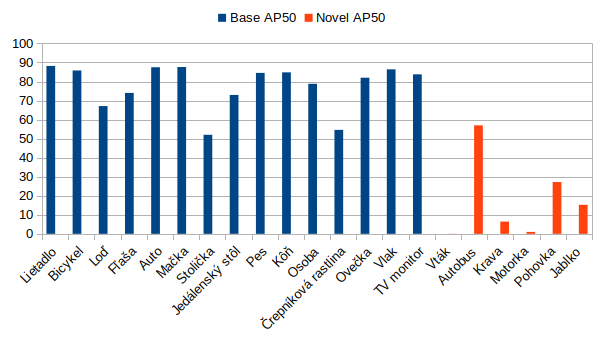
\includegraphics[width=\textwidth]{images/1_shot_classes_AP50.png}
\centering
\caption{AP50 na testovacích dátach pre jednotlivé triedy pre 1-shot detekciu.}
\label{fig:image18}
\end{figure}

\begin{figure}[H]
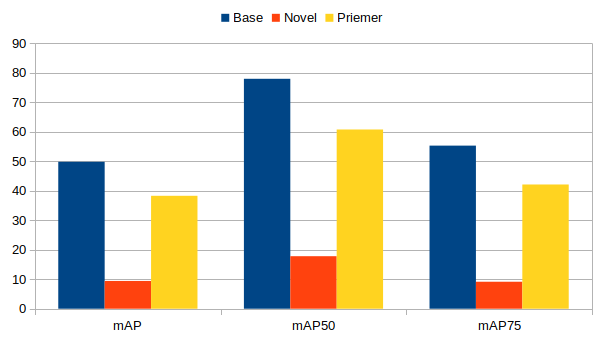
\includegraphics[width=\textwidth]{images/1_shot_meanAP.png}
\centering
\caption{Graf presností na testovacích dátach pre 1-shot detekciu.}
\label{fig:image20}
\end{figure}

\begin{table}[H]
\begin{tabular}{|l|c|c|c|}
\hline
\textbf{Presnosť} & \textbf{Base} & \textbf{Novel} & \textbf{Priemer} \\
\hline
mAP & 49.858 & 9.41 & 38.301 \\
mAP50 & 78.004 & 17.812 & 60.806 \\
mAP75 & 55.335 & 9.142 & 42.137 \\
\hline
\end{tabular}
\centering
\caption{Tabuľka presností na testovacích dátach pre 1-shot deketciu.}
\label{tab:table1}
\end{table}


\subsection{2-shot detekcia}

Celkový čas tréningu: 1 hodina, 51 minút a 41 sekúnd, na obrázku \ref{fig:image21} vidíme presnosť AP50 pre jednotlivé triedy, vidíme, že rozloženie presnosti sa zlepšila oproti 1-shot detekcii a už dokážeme rozpoznať každý objekt aspoň s nejakou presnosťou. Na obrázku \ref{fig:image23} a v tabuľke \ref{tab:table2} vidíme priemernú presnosť nášho modelu.

\begin{figure}[H]
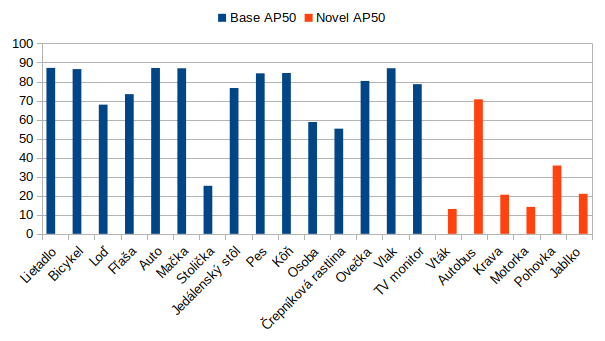
\includegraphics[width=\textwidth]{images/2_shot_classes_AP50.png}
\centering
\caption{AP50 na testovacích dátach pre jednotlivé triedy pre 2-shot detekciu.}
\label{fig:image21}
\end{figure}

\begin{figure}[H]
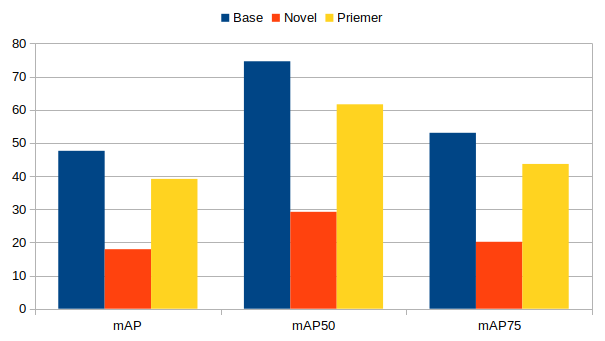
\includegraphics[width=\textwidth]{images/2_shot_meanAP.png}
\centering
\caption{Graf presností na testovacích dátach pre 2-shot detekciu.}
\label{fig:image23}
\end{figure}

\begin{table}[H]
\begin{tabular}{|l|c|c|c|}
\hline
\textbf{Presnosť} & \textbf{Base} & \textbf{Novel} & \textbf{Priemer} \\
\hline
mAP & 47.623 & 17.947 & 39.144 \\
mAP50 & 74.623 & 29.218 & 61.65 \\
mAP75 & 53.055 & 20.182 & 43.663 \\
\hline
\end{tabular}
\centering
\caption{Tabuľka presností na testovacích dátach pre 2-shot deketciu.}
\label{tab:table2}
\end{table}

\subsection{3-shot detekcia}

Celkový čas tréningu: 2 hodiny, 46 minút a 44 sekúnd, na obrázku \ref{fig:image25} vidíme presnosť AP50 pre jednotlivé triedy, vidíme, že rozloženie presnosti sa opäť zlepšilo, ale pre triedu vták je stále dosť nízka presnosť. Na obrázku \ref{fig:image27} a v tabuľke \ref{tab:table3} vidíme priemernú presnosť nášho modelu.

\begin{figure}[H]
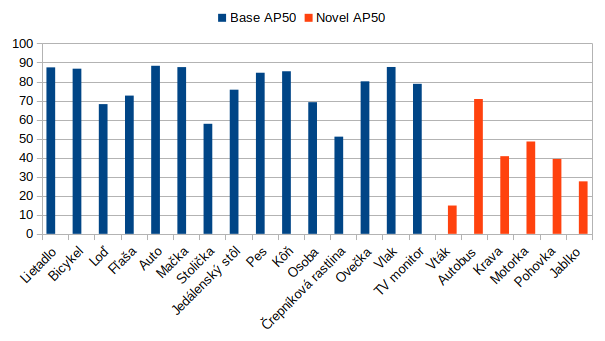
\includegraphics[width=\textwidth]{images/3_shot_classes_AP50.png}
\centering
\caption{AP50 na testovacích dátach pre jednotlivé triedy pre 3-shot detekciu.}
\label{fig:image25}
\end{figure}

\begin{figure}[H]
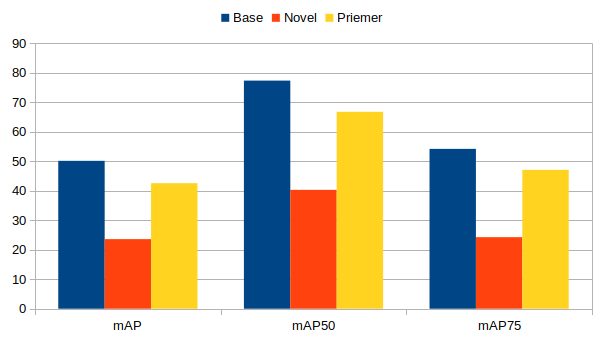
\includegraphics[width=\textwidth]{images/3_shot_meanAP.png}
\centering
\caption{Graf presností na testovacích dátach pre 3-shot detekciu.}
\label{fig:image27}
\end{figure}

\begin{table}[H]
\begin{tabular}{|l|c|c|c|}
\hline
\textbf{Presnosť} & \textbf{Base} & \textbf{Novel} & \textbf{Priemer} \\
\hline
mAP & 50.173 & 23.598 & 42.58 \\
mAP50 & 77.393 & 40.309 & 66.798 \\
mAP75 & 54.235 & 24.273 & 47.103 \\
\hline
\end{tabular}
\centering
\caption{Tabuľka presností na testovacích dátach pre 3-shot deketciu.}
\label{tab:table3}
\end{table}

\subsection{5-shot detekcia}

Celkový čas tréningu: 4 hodiny, 35 minút a 25 sekúnd. Ako vidíme tréningový čas nám veľmi rastie pri zvyšovaní počtu trénovacích obrázkov, keďže taktiež treba zvyšovať počet iterácií, aby sme dosiahli optimálne výsledky. Na obrázku \ref{fig:image28} vidíme presnosť AP50 pre jednotlivé triedy, vidíme, že rozloženie presnosti sa zvyšovaním počtu trénovacích obrázkov stále zvyšuje a tentokrát už máme pre každú triedu AP50 nad 30. Na obrázku \ref{fig:image30} a \ref{tab:table4} vidíme priemernú presnosť nášho modelu.

\begin{figure}[H]
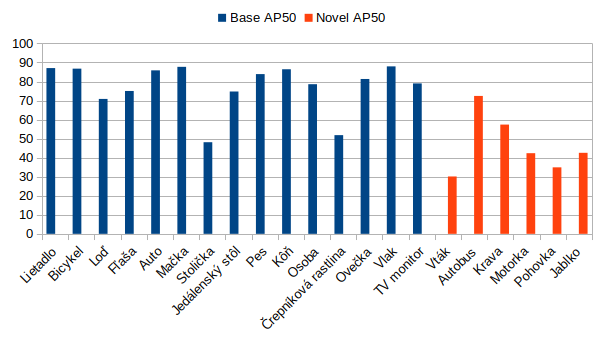
\includegraphics[width=\textwidth]{images/5_shot_classes_AP50.png}
\centering
\caption{AP50 na testovacích dátach pre jednotlivé triedy pre 5-shot detekciu.}
\label{fig:image28}
\end{figure}

\begin{figure}[H]
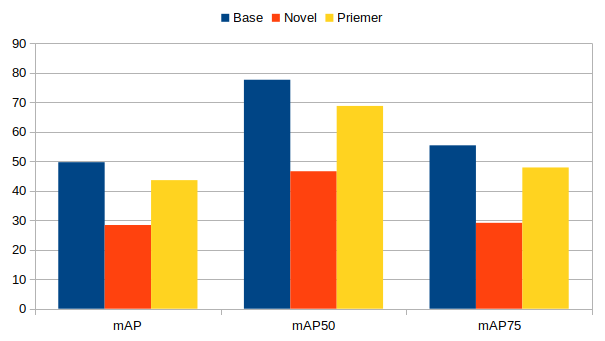
\includegraphics[width=\textwidth]{images/5_shot_meanAP.png}
\centering
\caption{Graf presností na testovacích dátach pre 5-shot detekciu.}
\label{fig:image30}
\end{figure}

\begin{table}[H]
\begin{tabular}{|l|c|c|c|}
\hline
\textbf{Presnosť} & \textbf{Base} & \textbf{Novel} & \textbf{Priemer} \\
\hline
mAP & 49.71 & 28.395 & 43.62 \\
mAP50 & 77.677 & 46.63 & 68.806 \\
mAP75 & 55.442 & 29.132 & 47.925 \\
\hline
\end{tabular}
\centering
\caption{Tabuľka presností na testovacích dátach pre 5-shot detekciu.}
\label{tab:table4}
\end{table}

\subsection{10-shot detekcia}

Celkový čas tréningu: 9 hodín, 11 minút a 4 sekundy. Na obrázku \ref{fig:image31} vidíme presnosť AP50 pre jednotlivé triedy. Na obrázku \ref{fig:image33} a v tabuľke \ref{tab:table5} vidíme priemernú presnosť nášho modelu.

\begin{figure}[H]
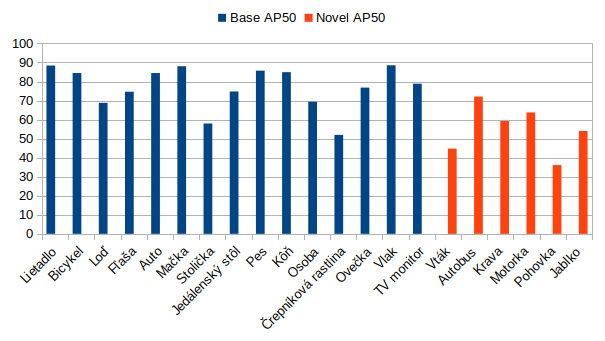
\includegraphics[width=\textwidth]{images/10_shot_classes_AP50.png}
\centering
\caption{AP50 na testovacích dátach pre jednotlivé triedy pre 10-shot detekciu.}
\label{fig:image31}
\end{figure}

\begin{figure}[H]
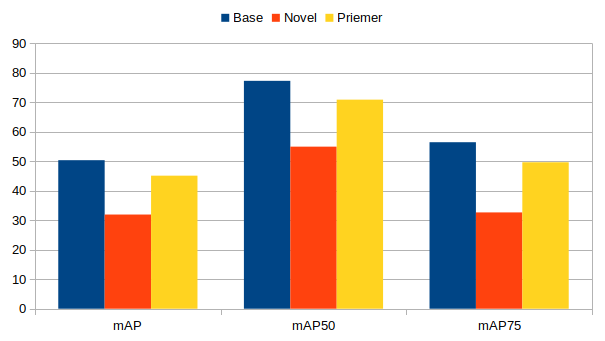
\includegraphics[width=\textwidth]{images/10_shot_meanAP.png}
\centering
\caption{Graf presností na testovacích dátach pre 10-shot detekciu.}
\label{fig:image33}
\end{figure}

\begin{table}[H]
\begin{tabular}{|l|c|c|c|}
\hline
\textbf{Presnosť} & \textbf{Base} & \textbf{Novel} & \textbf{Priemer} \\
\hline
mAP & 50.394 & 31.946 & 45.123 \\
mAP50 & 77.305 & 54.99 & 70.93 \\
mAP75 & 56.49 & 32.666 & 49.683 \\
\hline
\end{tabular}
\centering
\caption{Tabuľka presností na testovacích dátach pre 10-shot detekciu.}
\label{tab:table5}
\end{table}


\subsection{15-shot detekcia}

Celkový čas tréningu: 13 hodín, 56 minút a 37 sekúnd. Na obrázku \ref{fig:image34} vidíme presnosť AP50 pre jednotlivé triedy. Na obrázku \ref{fig:image36} a \ref{tab:table6} vidíme priemernú presnosť nášho modelu. Presnosť nášho modelu sa len minimálne zvýšila oproti 10-shot detekcii a pritom dĺžka tréningu sa zvýšila približne o 50 percent.

\begin{figure}[H]
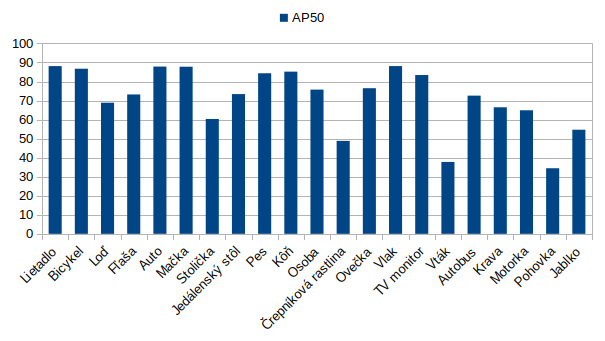
\includegraphics[width=\textwidth]{images/15_shot_classes_AP50.png}
\centering
\caption{AP50 na testovacích dátach pre jednotlivé triedy pre 15-shot detekciu.}
\label{fig:image34}
\end{figure}

\begin{figure}[H]
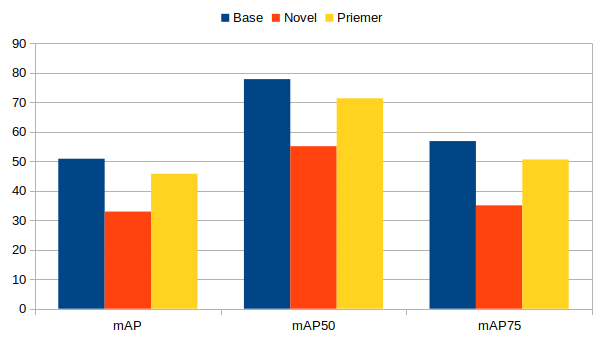
\includegraphics[width=\textwidth]{images/15_shot_meanAP.png}
\centering
\caption{Graf presností na testovacích dátach pre 15-shot detekciu.}
\label{fig:image36}
\end{figure}

\begin{table}[H]
\begin{tabular}{|l|c|c|c|}
\hline
\textbf{Presnosť} & \textbf{Base} & \textbf{Novel} & \textbf{Priemer} \\
\hline
mAP & 50.891 & 32.951 & 45.766 \\
mAP50 & 77.887 & 55.142 & 71.388 \\
mAP75 & 56.88 & 35.069 & 50.648 \\
\hline
\end{tabular}
\centering
\caption{Tabuľka presností na testovacích dátach pre 15-shot detekciu.}
\label{tab:table6}
\end{table}

\subsection{Vyhodnotenie}

Teraz vyhodnotíme rôzne vlastnosti fine-tuningu vzhľadom k počtu trénovacích obrázkov. 

\begin{figure}[H]
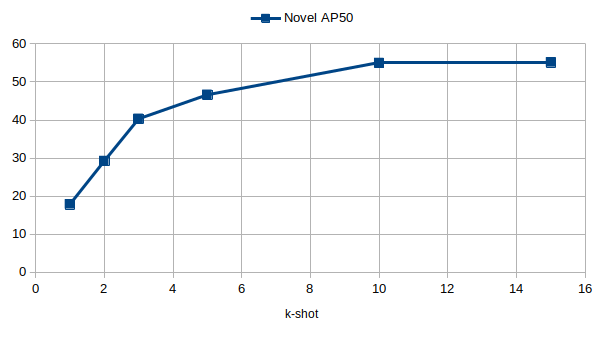
\includegraphics[width=\textwidth]{images/results_novel_AP50.png}
\centering
\caption{Novel AP50 na testovacích dátach vzhľadom k počtu trénovacích obrázkov.}
\label{fig:image37}
\end{figure}

Na obrázku \ref{fig:image37} vidíme presnosť novel tried vzhľadom k počtu trénovacíh obrázkov. Vidíme, že presnosť nám stále stúpa, ale po 10tich trénovacích obrázkoch nám presnosť stúpa už iba minimálne. Pri pätnástich trénovacích obrázkoch nám oproti desiatim stúpla presnosť iba o zanedbatelných 0.153.

\begin{figure}[H]
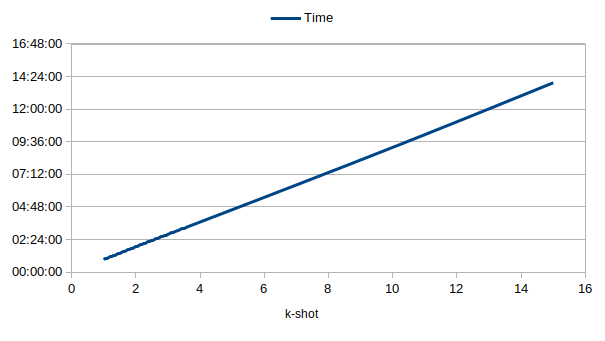
\includegraphics[width=\textwidth]{images/results_time.png}
\centering
\caption{Čas tréningu vzľadom k počtu trénovacích obrázkov.}
\label{fig:image38}
\end{figure}

Na ďaľšom obrázku \ref{fig:image38} vidíme ako sa nám mení čas tréningu, vzhľadom k počtu trénovacích obrázkov. Vidíme lineárnu funkciu, čas tréningu nám priamoúmerne stúpa s počtom trénovacích obrázkov.

\begin{figure}[H]
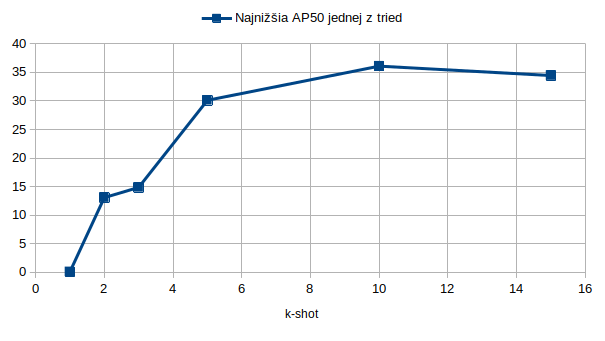
\includegraphics[width=\textwidth]{images/results_lowest_AP50.png}
\centering
\caption{Najnižia AP50 na testovacích dátach vzhľadom k počtu trénovacích obrázkov.}
\label{fig:image39}
\end{figure}

Ďalšia zaujímava metrika na obrázku \ref{fig:image39} nám ukazuje presnosť triedy s najmenšou presnosťou vzhľadom k počtu trénovacích obrázkov. Vidíme, že pri 1-shot detekcii jedna z tried má takmer nulovú presnosť, čo nie je úplne ideálne, keď je pre nás dôležité rozpoznávať všetky triedy. Tento graf nám teda zobrazuje garanciu najnižej presnosti pre každú z tried bez ohľadu na priemernú prenosť. Vidíme, že od 5-shot learningu máme celkom solidnú garanciu aspon 30 percent AP50 pre každú triedu. Pri 15-shot detekcii sa nám najnižia presnosť dokonca o trochu zníži oproti 10-shot detekcii, napriek jemnému zvýšeniu priemernej presnosti. 






